\chapter{آزمون چپمن-کولموگروف برای بازارهای مالی}
\label{ch4} 

از میان سیستم‌هایی که در زندگی انسان تاثیر گذار هستند، 
بازارهای مالی یکی از پیچیده‌ترین رفتارها را دارند و از آن‌ها به عنوان 
یک سیستم پیچیده نامبرده می‌شود. یکی از مباحث مهم در 
بازارهای مالی پیش‌بینی آینده یک سهم یا شاخص در بازارهای مالی است. 
رفتار تصادفی بازارهای مالی باعث شده است که بعضی از تحلیل‌گران 
بازارهای مالی از فرایند‌های تصادفی برای تحلیل بازار استفاده کنند.\cite{paul_stochastic_2013}
% به دلیل جذابیت بالای بازارهای مالی باعث شد 
% تا آزمون چپمن-کولموگروف برای دو فرایند‌ جفت‌شده را برای داده‌های 
% چند بازار مختلف بررسی کنیم.
رفتار بازارهای مالی در واقع برآمده از رفتار جمعی 
معامله کنندگان بازارهای مالی است که رفتار معامله کنندگان 
خود وابسته به عوامل بلند مدت و کوتاه مدت است. عوامل بلند مدتی همچون 
سیاست‌های کلان اقتصادی یک کشور می‌تواند بر رفتار یک بازار مالی در بلند 
مدت تاثیر بسزایی داشته باشد.
بنابراین دور از ذهن نیست که رفتار بازارهای مالی با زمان تغییراتی داشته باشد بنابراین 
برا محاسبه طول مارکوف بهتر است که این موضوع در نظر گرفته شود.

 \section{آماده سازی داده‌ها}

برای انجام آزمون چپمن-کولموگروف روی داده‌های بازارهای مالی دو رمزارز\LTRfootnote{Cryptocurrency} از بازار رمزها انتخاب شده است. 
% برای بررسی 
به طور دقیق‌تر برای محاسبه طول مارکوف از قیمت 
 قراردادهای دائمی\LTRfootnote{Perpetual contracts} صرافی بیتمِکس\LTRfootnote{Bitmex} 
برای رمز ارز بیتکوین\LTRfootnote{‌Bitcoin} و اتریوم \LTRfootnote{Ethereum}   
 استفاده شده است.\cite{bitmex} داده‌های مورد استفاده داده‌های تک‌تک معاملات 
قراردادهای دائمی این دو رمز ارز است که با نماد \lr{XBT/USD} و \lr{ETH/USD} شناخته می‌شوند. 
این داده‌ها متعلق به بازه سه ماهه از ابتدای ماه می 2020 تا انتهای جولای 2020 است.
با استفاده از قیمت تک‌تک معاملات در نهایت قیمت پایانی برای این قراردادها در هر ثانیه محاسبه 
شد که در شکل \ref{fig:XBTETH} روند کلی این دو رمزارز در بازه سه ماهه 
ماه می تا جولای نشان داده شده است.
\begin{figure}[H]
    \centering
    % \vspace{1cm}
    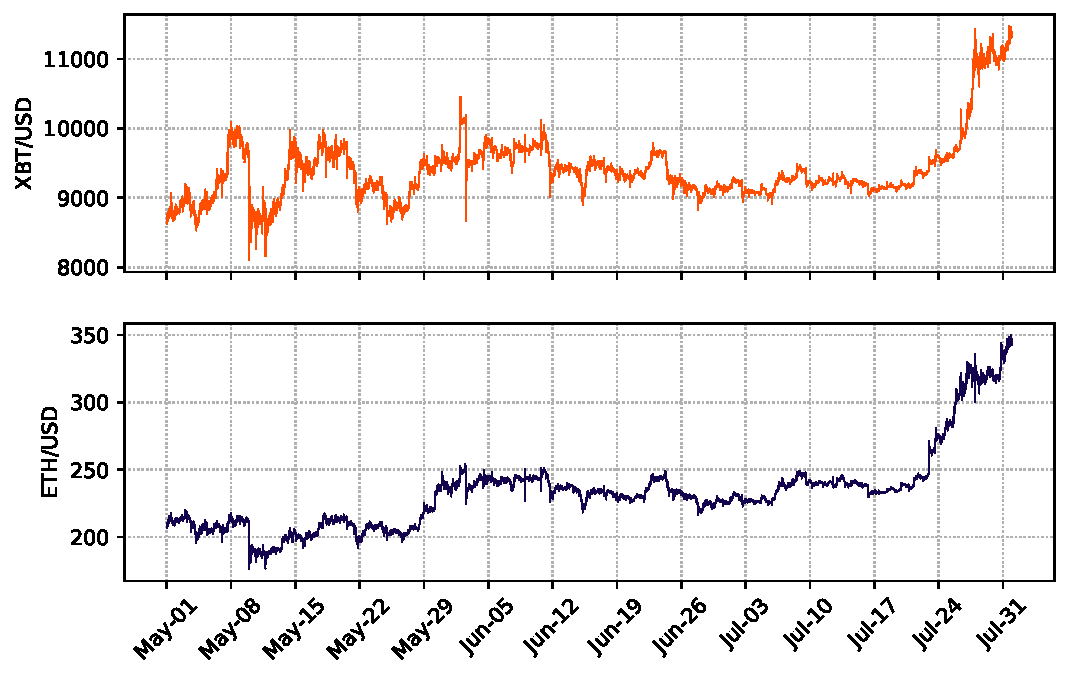
\includegraphics[width=0.7\textwidth]{images/xbteth.pdf}
    \caption{قیمت قراردادهای دائمی بیتکوین و اتریوم بر حسب دلار آمریکا در صرافی بیتمکس در بازه سه ماهه می تا جولای 2020.}\label{fig:XBTETH}
\end{figure}
% \begin{figure}[H]
%     \centering
%     % \vspace{1cm}
%     \subcaptionbox{جفت ارزهای یورو به دلار \lr{EUR/USD} و پوند به دلار \lr{GBP/USD} در ۱۸ می ۲۰۲۰.\label{fig:CCKtestyx}}
%     {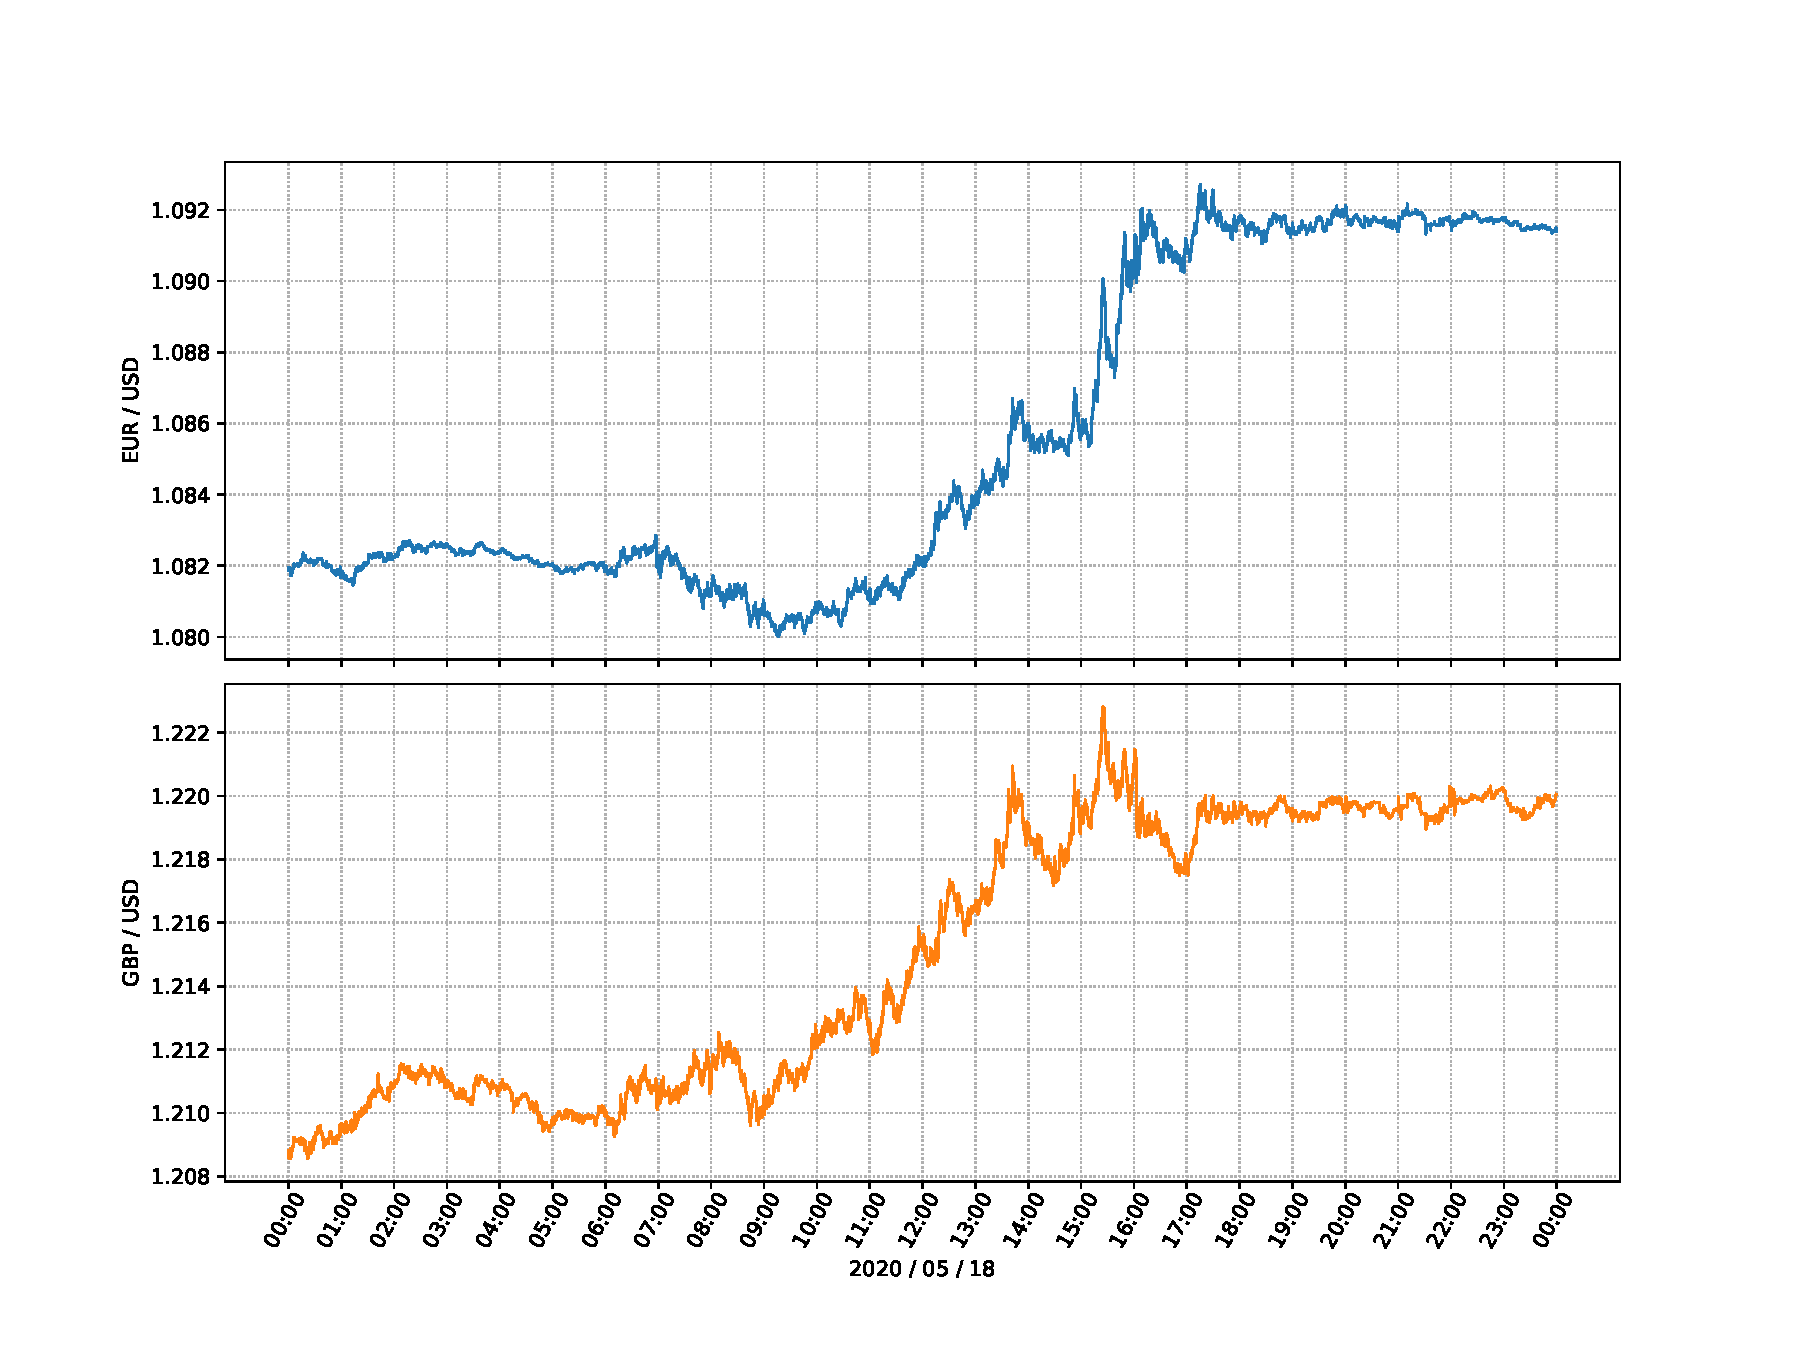
\includegraphics[width=0.49\textwidth]{images/EURGBP.pdf}}
%     \subcaptionbox{قیمت انس نقره به دلار \lr{XAG/USD} و قیمت انس طلا به دلار \lr{XAU/USD} در ۱۸ می ۲۰۲۰.\label{fig:CCKtestyy}}
%     {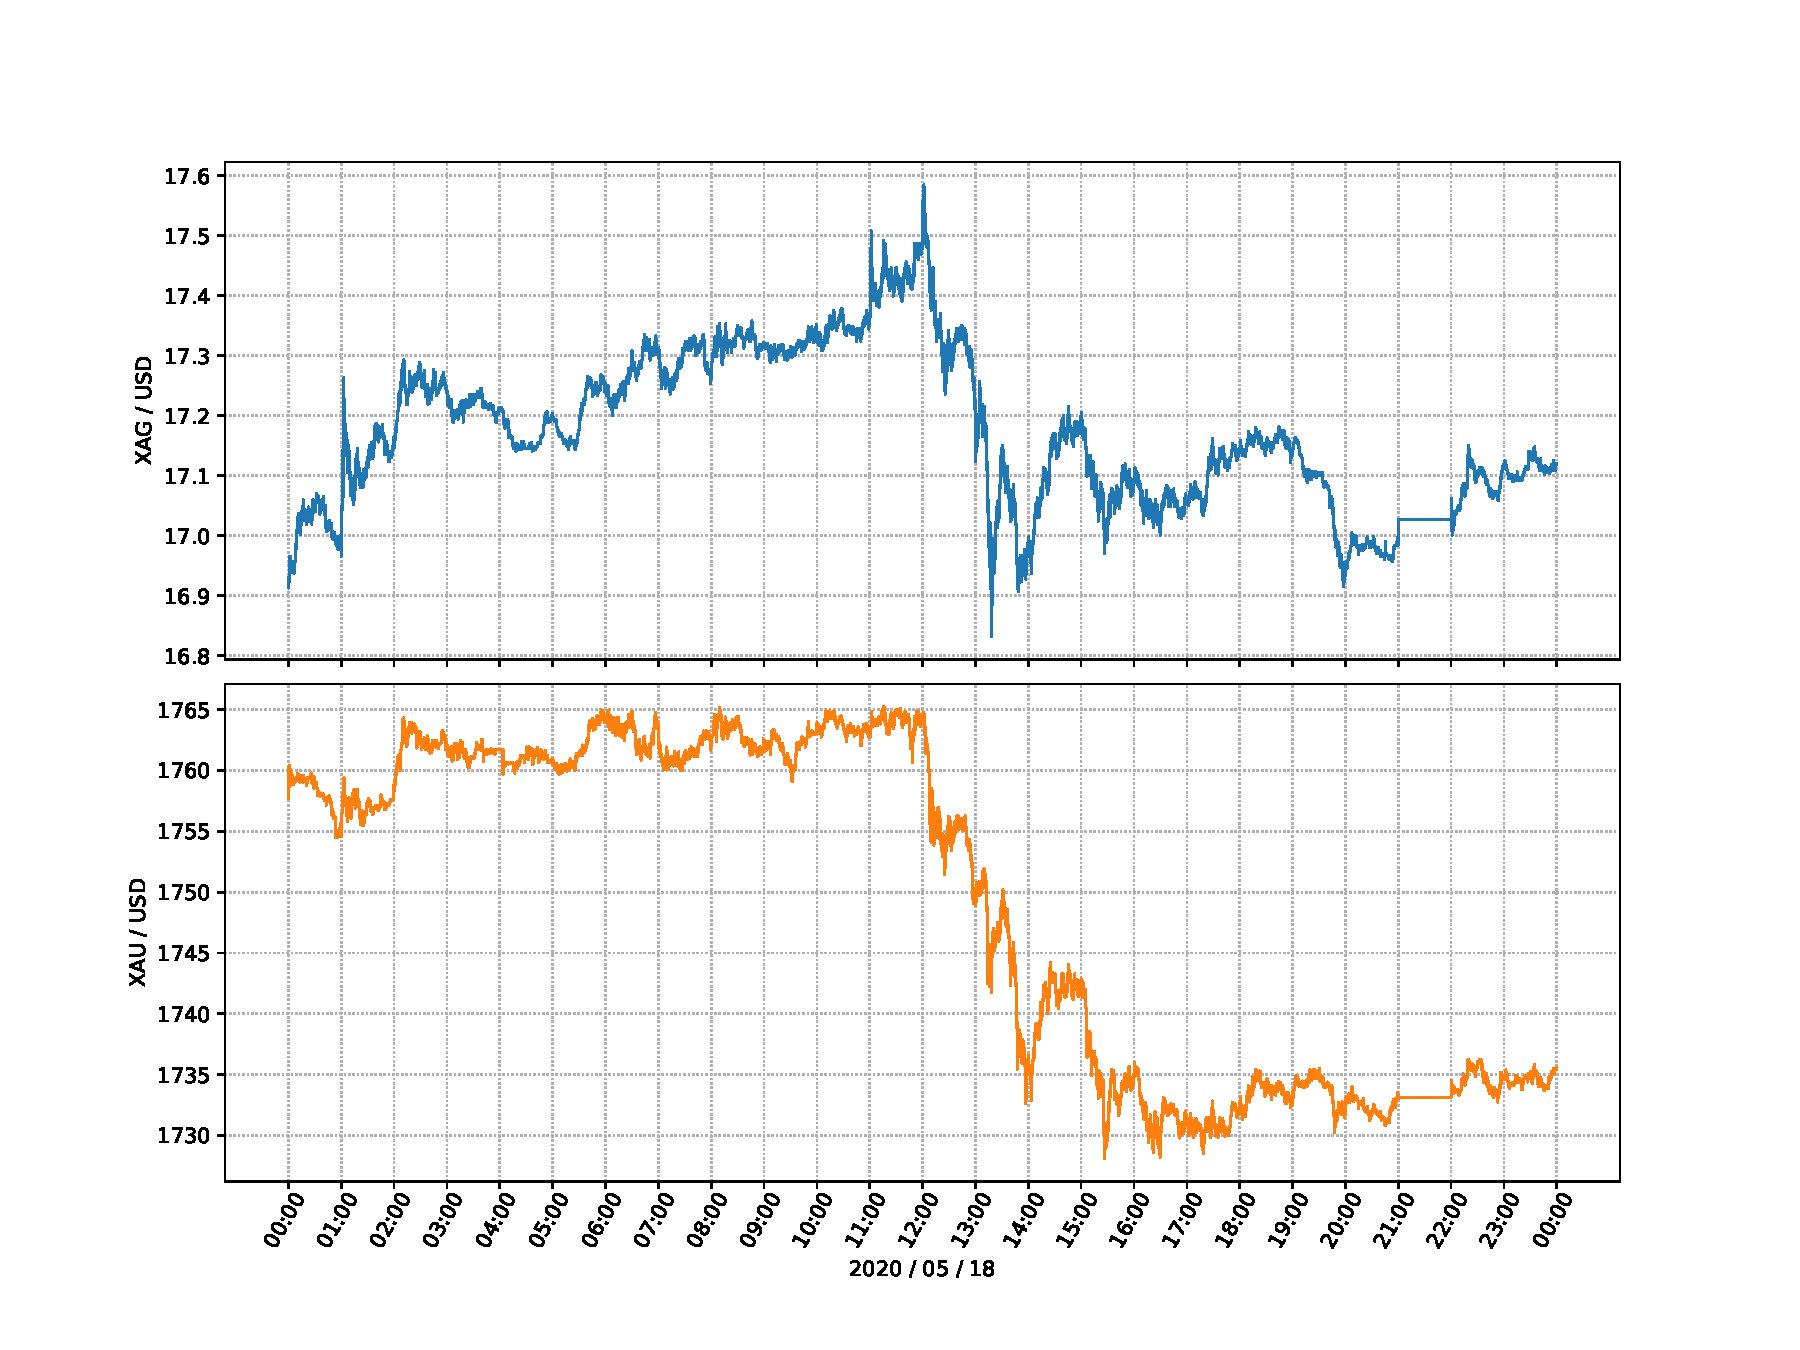
\includegraphics[width=0.49\textwidth]{images/XAGXAU.pdf}}
%     \caption{}\label{fig:CCKtesty}
% \end{figure}
برای محاسبه طول مارکوف با استفاده از آزمون 
چپمن-کولموگروف از بازده لگاریتمی\LTRfootnote{Logarithmic return} استفاده شده است. فرض کنید $x(t)$ 
یک شاخص یا قیمت یک سهم در یک بازار مالی باشد بازده لگاریتمی به شکل زیر محاسبه می‌شود. 
\begin{equation}
    r_x(t) = \ln \left( \frac{x(t+1)}{x(t)} \right)
\end{equation}
در رابطه بالا $r_x ( t )$ نشان‌ دنده بازده لگاریتمی است. 
دلیل استفاده از بازده لگاریتمی این است که در قدم اول $x(t+1)/x(t)$ نسبت تغییرات 
قیمت را نسبت به زمان قبل می‌دهد و با گرفتن لگاریتم از این مقادیر می‌توانیم نسبت تغییرات را حول 
صفر داشته باشیم. در واقع با محاسبه بازده لگاریتمی می‌توانیم داده‌هایی با میانگین نزدیک به صفر داشته 
باشیم که می‌توانیم آن‌ها را مانا فرض کنیم.
 
 \section{محاسبه طول مارکوف داده‌های مالی}
 همانطور که قبلا اشاره شده ممکن است رفتار بازارهای مالی با زمان تغییر کند و محاسبه طول مارکوف 
 برای بازه‌های زمانی طولانی مثلا سالانه یا ماهانه چندان مفید به نظر نمی‌رسد. بنابراین بهتر است که 
تخمین طول مارکوف را در بازه‌های کوتاه‌تر مثل هفتگی یا روزانه انجام داد اما از طرفی باید در نظر داشت 
که هرچه بازه زمانی کوتاه‌تر باشد تعداد نقاط سری‌های زمانی هم کمتر خواهد شد و توزیع چگالی‌های به دست آمده 
از این سری‌های زمانی خطای زیادی خواهد داشت. در این تحقیق از بازه زمانی هفت روزه استفاده شده است 
که در حدود $6 \times 10^5$ ثانیه است. در ادامه نتیجه آزمون چپمن-کولموگروف برای چند بازه هفت روزه 
آورده شده است. شکل زیر هم نمودار انحراف معیار بازده‌های لگاریتمی\LTRfootnote{Volatility} $r_x(t)$ و 
$r_y(t)$ است که $r_x(t)$ بازده لگاریتمی بیتکوین و $r_y(t)$ بازده لگاریتمی اتریوم است. 
در شکل زیر $\sigma_{XBT}(t)$ نشان دهنده انحراف معیار بیتکوین در بازه هفتگی است که ابتدای آن در $t$ 
قرار دارد و $\sigma_{XBT}$ نشان دهنده انحراف معیار کل بازه سه ماهه است. کمیت‌های مشابه برای اتریوم با 
$\sigma_{ETH}(t)$ و $\sigma_{ETH}$ نشان داده شده‌اند.
بازه‌های هفت روزه در طول بازه سه ماهه از می تا جولای 2020 
است که به عنوان معیاری از بزرگی نوسان قیمت در در نظر گرفته شده است.

\begin{figure}[H]
    \centering
    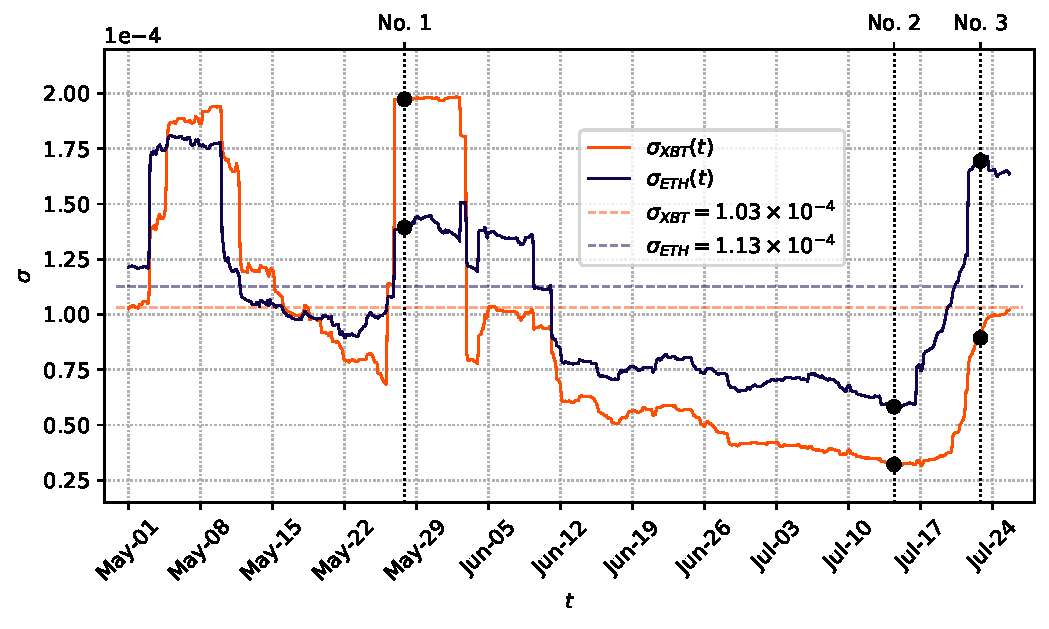
\includegraphics[width=\textwidth]{images/xbteth_volatility.pdf}
    \caption{نمودار انحراف معیار بازده‌های لگاریتمی $r_x(t)$ و $r_y(t)$ در بازه‌های هفت روزه در طول بازه سه ماهه از می تا جولای 2020.}\label{fig:xbteth_volatility}
\end{figure}
به عنوان نمونه، برای سه بازه هفتگی زیر نتایج تخمین طول ماروکوف آورده شده است که در ادامه به آن می‌پردازیم. مقدار انحراف معیار در این بازه‌ها در شکل \ref{fig:xbteth_volatility} 
با شماره‌های ۱ تا ۳ نشان داده شده‌اند.
\begin{table}[htb]
    \centering
    \caption{سه بازه هفتگی که برای محاسبه طول ماروکوف استفاده شده‌اند.\label{interval_table}}
    \begin{tabular}{|c|c|c|c|}
      \hline
      \cellcolor[HTML]{C0C0C0}& بازه & $\sigma_{XBT}(t)$ & $\sigma_{ETH}(t)$\\ \hline
        ۱ & ۲۷ می ۱۳:۳۳:۲۰ تا ۳ جون ۱۳:۳۳:۲۰ & $1.97 \times 10^{-4}$ & $1.39 \times 10^{-4}$ \\ \hline
        ۲ & ۱۳ جولای ۱۹:۳۴:۱۳ تا ۲۰ جولای ۱۹:۳۴:۱۳ & $3.22 \times 10^{-5}$ & $5.67 \times 10^{-5}$ \\ \hline
        ۳ & ۲۲ جولای ۲:۵۳:۲۰ تا ۲۹ جولای ۲:۵۳:۲۰ & $8.93 \times 10^{-5}$ & $1.69 \times 10^{-4}$\\ \hline
      \end{tabular}
  \end{table}
  \FloatBarrier

\subsubsection{محاسبه طول مارکوف در بازه شماره ۱}
همانطور که در جدول \ref{interval_table} آمده است بازه شماره ۱ از تاریخ ۲۷ می ۲۰۲۰ ساعت ۱۳:۳۳:۲۰ تا ۳ جون ۲۰۲۰ و تا همان ساعت است. 
مقدار انحراف معیار بیتکوین در این بازه برابر $1.97 \times 10^{-4}$ و انحراف معیار اتریوم برابر با $1.39 \times 10^{-4}$ 
است. نوسان قیمت بیتکوین و اتریوم در این بازه در شکل زیر آورده شده است. دلیل انتخاب این بازه این است که مقدار انحراف معیار بیتکوین یکی بیشترین مقادیر 
در بین بازه‌های دیگر را دارد.
\begin{figure}[H]
  \centering
  % \vspace{1cm}
  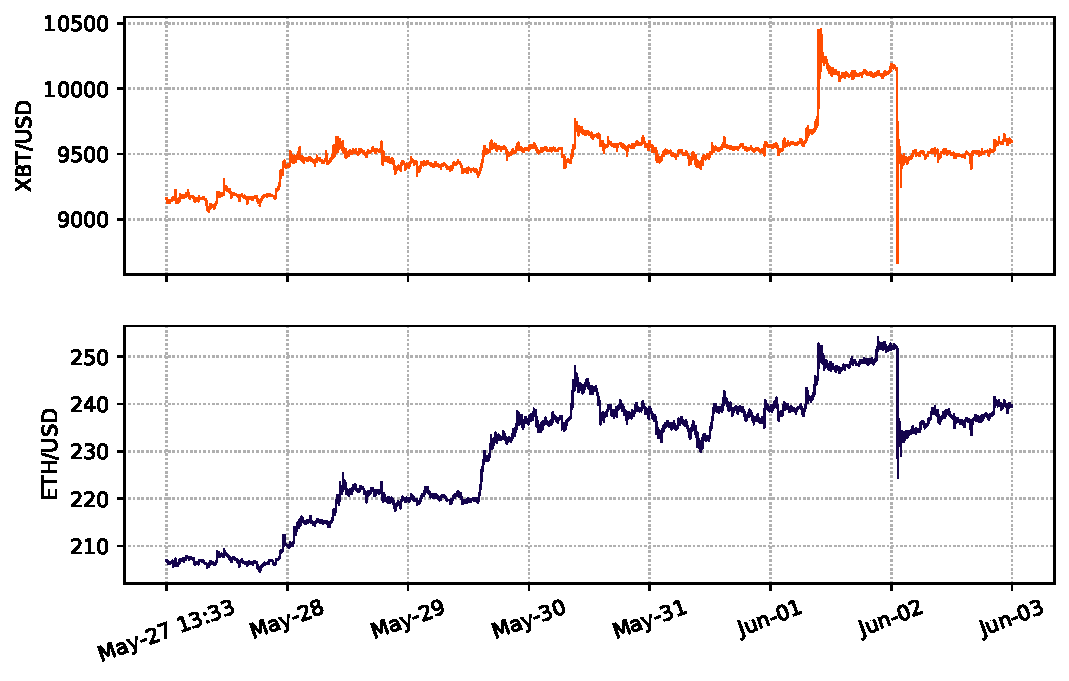
\includegraphics[width=\textwidth]{images/xbteth1.pdf}
  \caption{قیمت قراردادهای دائمی بیتکوین و اتریوم بر حسب دلار آمریکا در بازه شماره ۱.}\label{fig:XBTETH1}
\end{figure}

\begin{figure}[H]
  \centering
  \subcaptionbox{در این شکل $S_1$ نشان دهنده طول مارکوف بیتکوین به خودش است، $l_1 = 526$.\label{fig:ckxbteth11}}
  {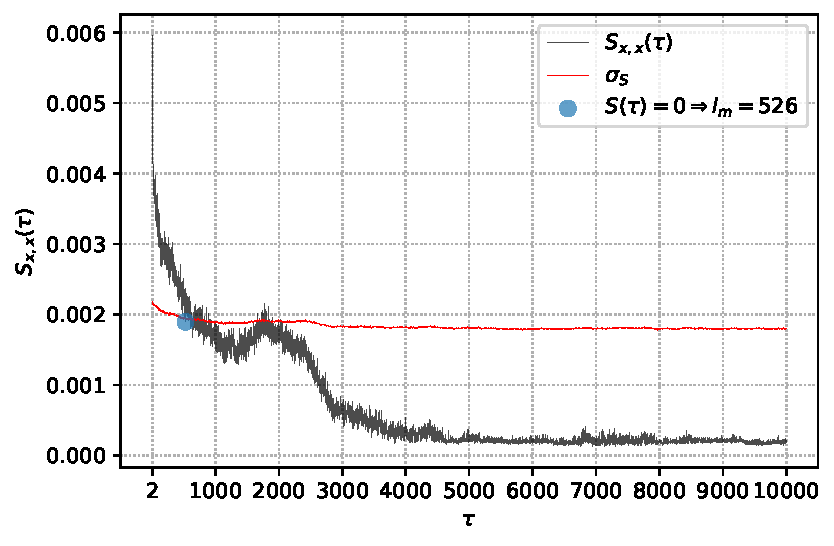
\includegraphics[width=0.49\textwidth]{images/no1_0.pdf}}
  \subcaptionbox{در این شکل $S_2$ نشان دهنده طول مارکوف بیتکوین به اتریوم است، $l_2 = 302$.\label{fig:ckxbteth12}}
  {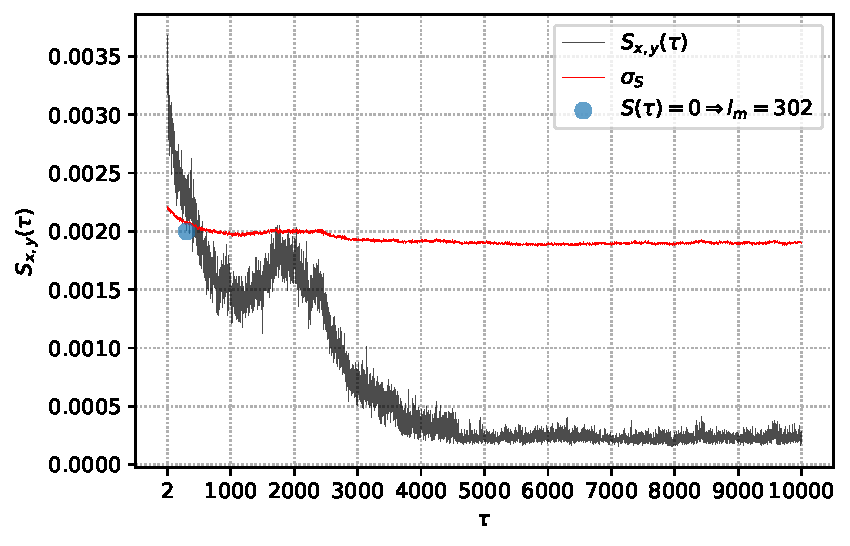
\includegraphics[width=0.49\textwidth]{images/no1_1.pdf}}
  \subcaptionbox{در این شکل $S_3$ نشان دهنده طول مارکوف اتریوم به بیتکوین است، $l_3 = 313$.\label{fig:ckxbteth13}}
  {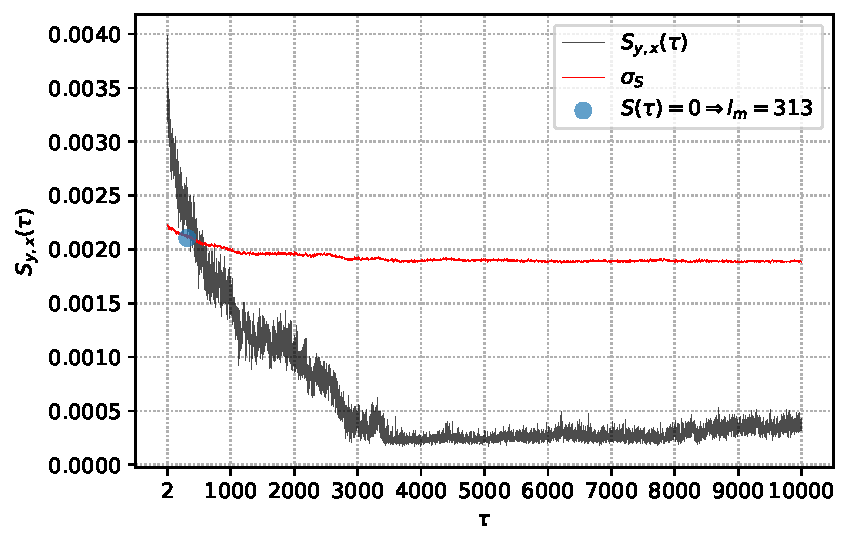
\includegraphics[width=0.49\textwidth]{images/no1_2.pdf}}
  \subcaptionbox{در این شکل $S_4$ نشان دهنده طول مارکوف اتریوم به خودش است، $l_4 = 436$.\label{fig:ckxbteth14}}
  {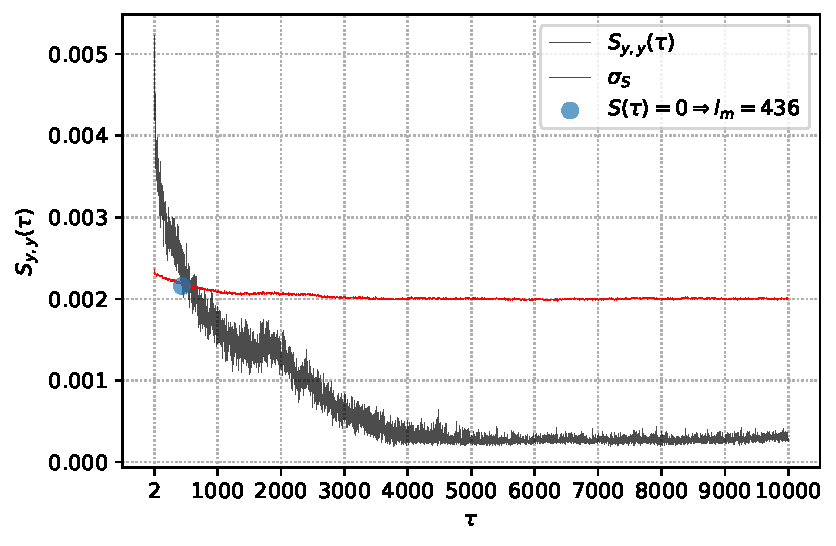
\includegraphics[width=0.49\textwidth]{images/no1_3.pdf}}
  \caption{نمودار آزمون چپمن-کولموگروف برای بیتکوین و اتریوم در بازه شماره ۱.}\label{fig:ckxbteth1}
\end{figure}
در شکل \ref{fig:ckxbteth1} مقادیر $S_1( \tau )$، $S_2( \tau )$، $S_3( \tau )$ و $S_4( \tau )$ برحسب $\tau$ 
کشیده شده‌اند این مقادیر به ترتیب نشان دهنده وابستگی نوسان قیمت بیتکوین به خودش و اتریوم و نوسان قیمت اتریوم به بیتکوین و خودش هستند. 
همانطور که در شکل \ref{fig:ckxbteth11} پیداست مقدار $S_1( \tau )$ در $\tau = 527$ با در نظر گرفتن خطا 
صفر شده است. از شکل \ref{fig:ckxbteth12} نیز پیداست که $S_2( \tau )$ در $\tau = 303$ با در نظر گرفتن خطا صفر شده است. 
بنابراین برای این بازه $l_1 = 526$ ثانیه و $l_2 = 302$ ثانیه به دست می‌آیند که طول مارکوف بیتکوین نسبت به خودش و اتریوم در این بازه هستند. در شکل 
\ref{fig:ckxbteth14} طول مارکوف اتریوم نسبت به خودش یعنی $l_4$ برابر با $436$ به دست آمده است و 
در شکل \ref{fig:ckxbteth13} $l_3$ که طول مارکوف اتریوم نسبت به بیتکوین است برابر با $313$ به دست آمده است.


\subsubsection{محاسبه طول مارکوف در بازه شماره ۲}
بازه شماره ۲ از تاریخ ۱۳ جولای ۲۰۲۰ ساعت ۱۹:۳۴:۱۳ تا ۲۰ جولای ۲۰۲۰ و تا همان ساعت است. 
مقدار انحراف معیار بیتکوین در این بازه برابر $3.22 \times 10^{-5}$ و انحراف معیار اتریوم برابر با $5.67 \times 10^{-5}$ 
است. این بازه به این دلیل انتخاب شده ‌است که انحراف معیار بیتکوین در این بازه کمینه شده است.

در شکل \ref{fig:ckxbteth2} نتیجه آزمون چپمن-کولموگروف در این بازه نشان داده شده است. 
با توجه به شکل‌های \ref{fig:ckxbteth21}، \ref{fig:ckxbteth22} و \ref{fig:ckxbteth23} مقادیر $S_1(\tau)$، $S_2(\tau)$ و $S_3(\tau)$ 
در $\tau = 2$ با در نظر گرفتن خطا صفر شده‌اند که این مقدار $\tau$ با توجه به \ref{coupled_cktest} نشان دهنده این است که طول مارکوف بیتکوین نسبت به خودش و 
اتریوم و همچنین اتریوم نسبت به بیتکوین در این بازه کمتر از $1$ است. با توجه به شکل \ref{fig:ckxbteth24} تنها طول مارکوف اتریوم نسبت به 
خودش برابر با $5$ ثانیه است.
\begin{figure}[H]
  \centering
  % \vspace{1cm}
  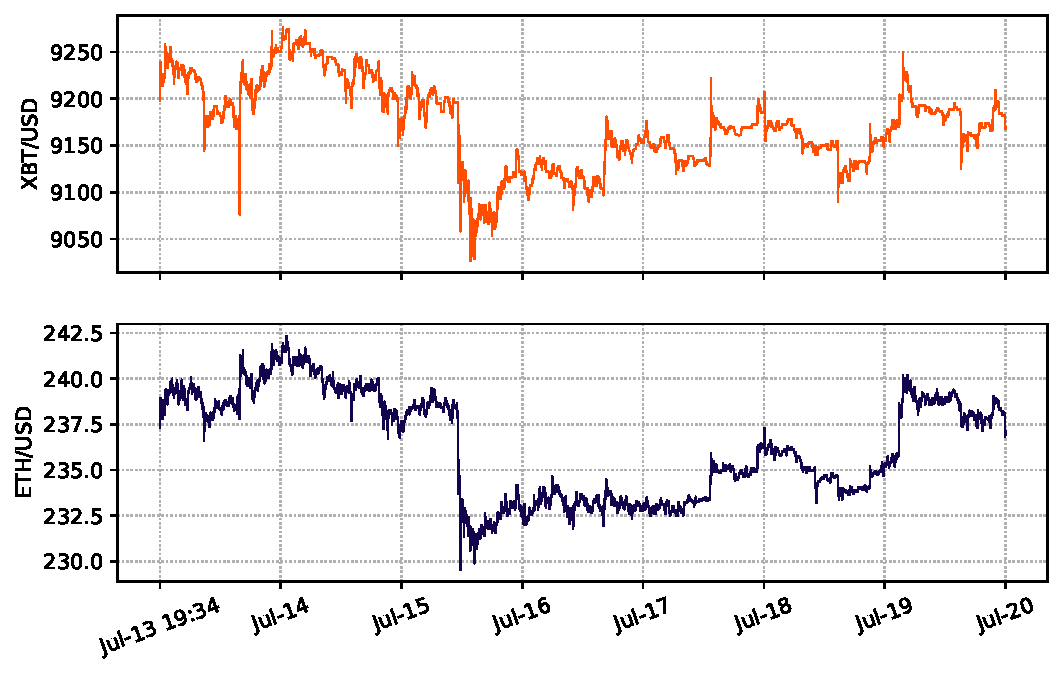
\includegraphics[width=\textwidth]{images/xbteth2.pdf}
  \caption{قیمت قراردادهای دائمی بیتکوین و اتریوم بر حسب دلار آمریکا در بازه شماره ۲.}\label{fig:XBTETH2}
\end{figure}
\begin{figure}[H]
    \centering
    \subcaptionbox{در این شکل $S_1$ نشان دهنده طول مارکوف بیتکوین به خودش است، $l_1 \leq 1$.\label{fig:ckxbteth21}}
    {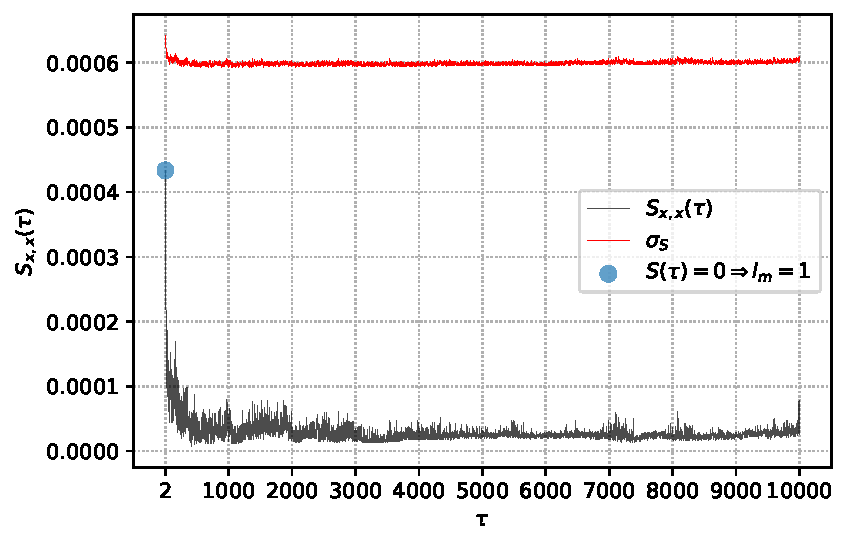
\includegraphics[width=0.49\textwidth]{images/no2_0.pdf}}
    \subcaptionbox{در این شکل $S_2$ نشان دهنده طول مارکوف بیتکوین به اتریوم است، $l_2 \leq 1$.\label{fig:ckxbteth22}}
    {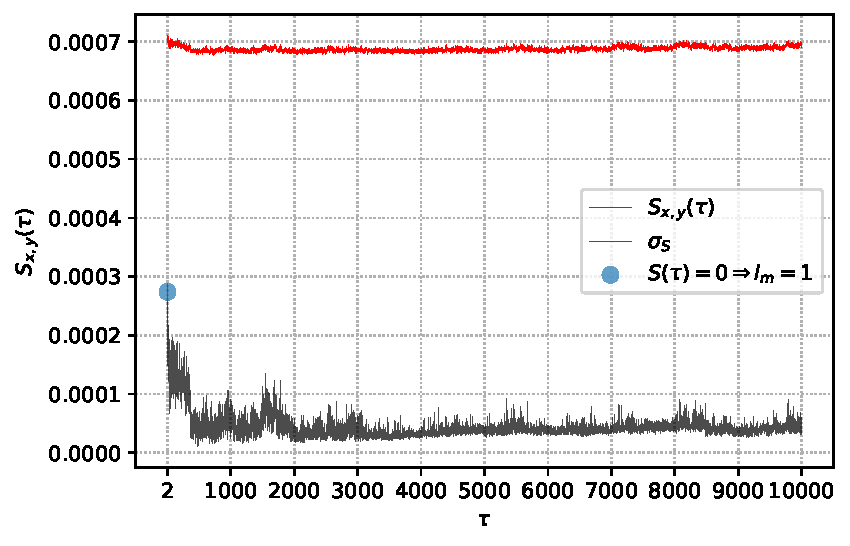
\includegraphics[width=0.49\textwidth]{images/no2_1.pdf}}
    \subcaptionbox{در این شکل $S_3$ نشان دهنده طول مارکوف اتریوم به بیتکوین است، $l_3 \leq 1$.\label{fig:ckxbteth23}}
    {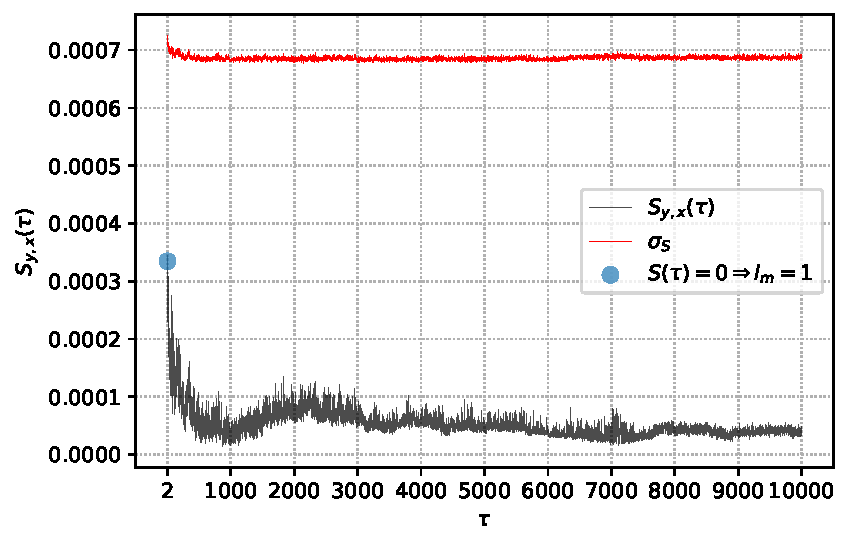
\includegraphics[width=0.49\textwidth]{images/no2_2.pdf}}
    \subcaptionbox{در این شکل $S_4$ نشان دهنده طول مارکوف اتریوم به خودش است، $l_4 = 5$.\label{fig:ckxbteth24}}
    {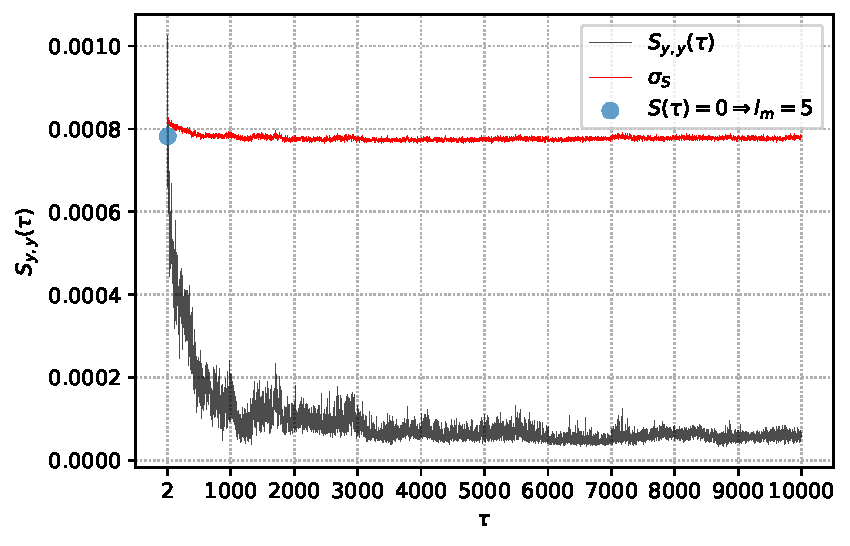
\includegraphics[width=0.49\textwidth]{images/no2_3.pdf}}
    \caption{نمودار آزمون چپمن-کولموگروف برای بیتکوین و اتریوم در بازه شماره ۲.}\label{fig:ckxbteth2}
\end{figure}

\subsubsection{محاسبه طول مارکوف در بازه شماره ۳}
بازه شماره ۳ از تاریخ ۲۲ جولای ۲۰۲۰ ساعت ۲:۵۳:۲۰ تا ۲۹ جولای ۲۰۲۰ است. 
مقدار انحراف معیار بیتکوین در این بازه برابر $8.93 \times 10^{-5}$ و انحراف معیار اتریوم برابر با $1.69 \times 10^{-4}$ 
است. نوسان قیمت بیتکوین و اتریوم در این بازه در شکل \ref{fig:XBTETH3} آورده شده است. این بازه به این دلیل انتخاب شده است که انحراف معیار بیتکوین 
در این بازه کمتر از انحراف معیار سه ماهه بیتکوین است و انحراف معیار اتریوم بیشتر از انحراف معیار سه ماهه است.

در شکل \ref{fig:ckxbteth3} نتیجه آزمون چپمن-کولموگروف برای بازه شماره ۳ رسم شده است. 
با توجه به شکل‌های \ref{fig:ckxbteth31} و \ref{fig:ckxbteth32} طول مارکوف بیتکوین نسبت به خودش و 
اتریوم یعنی $l_1$ و $l_2$ به ترتیب $1371$ و $483$ ثانیه به دست آمده‌اند. همچنین با توجه به شکل‌های \ref{fig:ckxbteth33} و 
\ref{fig:ckxbteth34} طول مارکوف اتریوم نسبت به بیتکوین $l_3 = 597$ ثانیه و طول مارکوف اتریوم نسبت به خودش 
$l_4=2012$ ثانیه به دست آمده‌اند.

\begin{figure}[H]
  \centering
  % \vspace{1cm}
  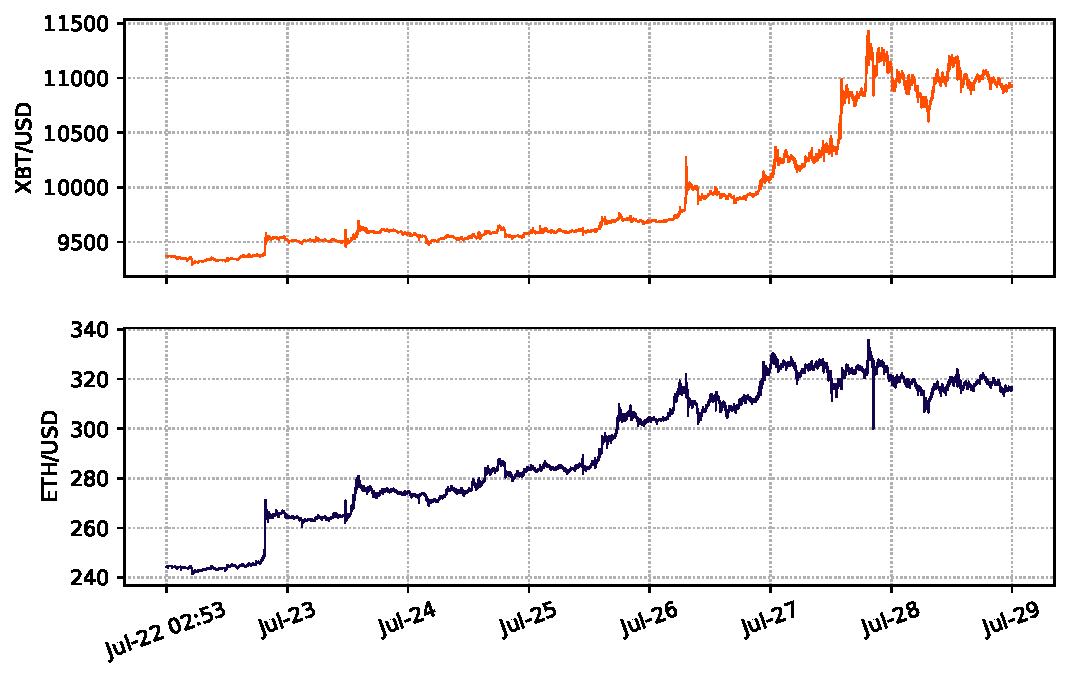
\includegraphics[width=0.7\textwidth]{images/xbteth3.pdf}
  \caption{قیمت قراردادهای دائمی بیتکوین و اتریوم بر حسب دلار آمریکا در بازه شماره ۳.}\label{fig:XBTETH3}
\end{figure}

\begin{figure}[H]
    \centering
    \subcaptionbox{$S_1( \tau ), l_1 = 1371$.\label{fig:ckxbteth31}}
    {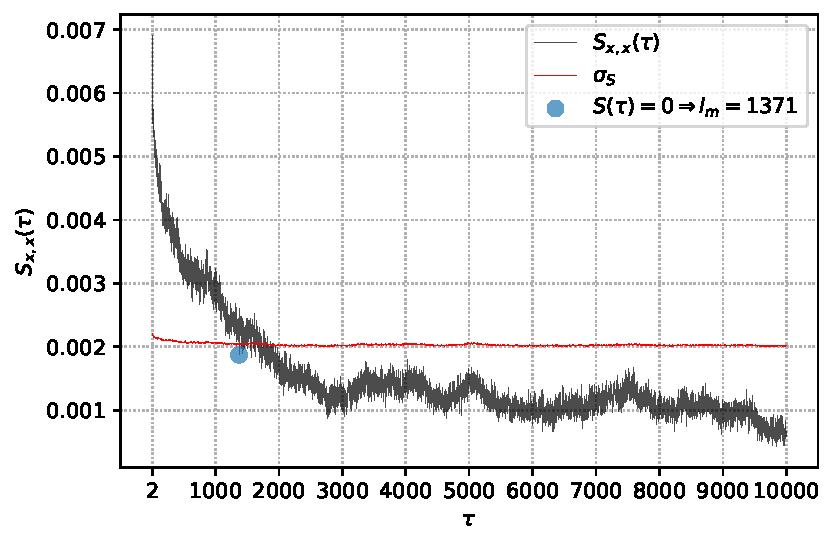
\includegraphics[width=0.49\textwidth]{images/no3_0.pdf}}
    \subcaptionbox{$S_2( \tau ), l_2 = 483$.\label{fig:ckxbteth32}}
    {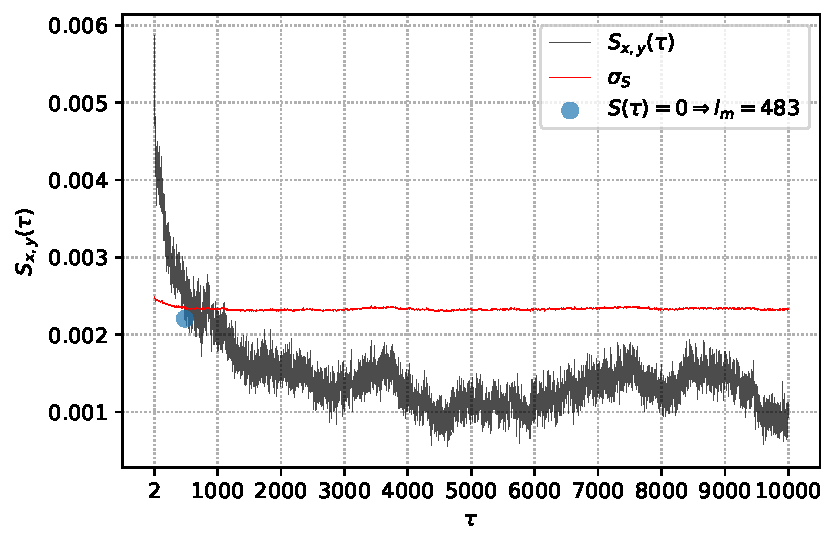
\includegraphics[width=0.49\textwidth]{images/no3_1.pdf}}
    \subcaptionbox{$S_3( \tau ), l_3 = 597$.\label{fig:ckxbteth33}}
    {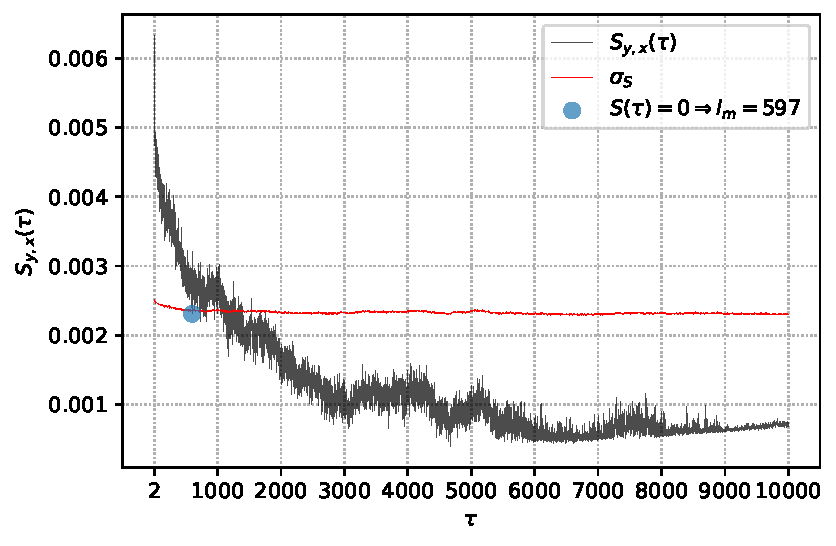
\includegraphics[width=0.49\textwidth]{images/no3_2.pdf}}
    \subcaptionbox{$S_4( \tau ), l_4 = 2012$.\label{fig:ckxbteth34}}
    {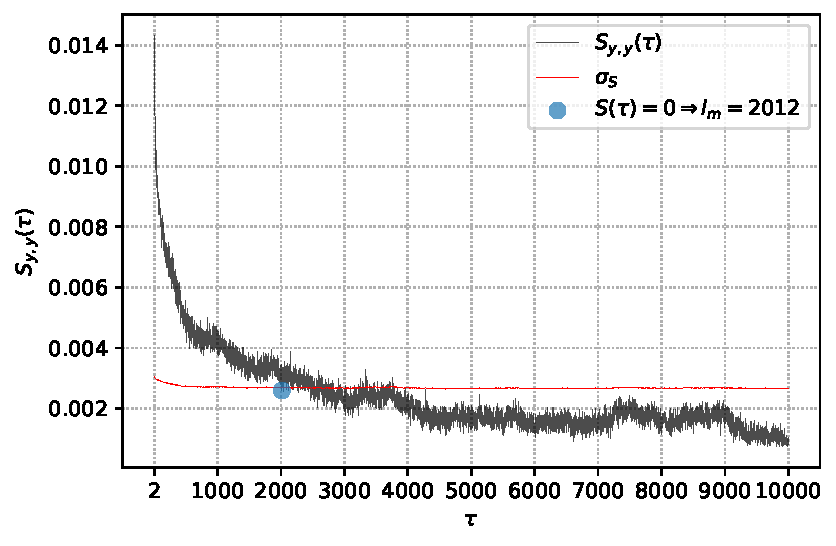
\includegraphics[width=0.49\textwidth]{images/no3_3.pdf}}
    \caption{نمودار آزمون چپمن-کولموگروف برای بیتکوین و اتریوم در بازه شماره ۳.}\label{fig:ckxbteth3}
\end{figure}